\section{Definition of an Event Tree}
\label{sec:event_tree_definition}

An \acrfull{et} unravels how a single \emph{initiating event} (\(I\)) can branch into multiple possible \emph{end-states} (\(X\)) through a sequence of \emph{functional} (or conditional) events. Each branch captures the success or failure of an important \emph{functional event} (e.g.\ a safety barrier or operator intervention). By following all possible paths, one can systematically account for each final outcome \(X_j\). Figure~\ref{fig:event_tree_example} provides a schematic view of this process for an initiating event \(I\) and two subsequent functional events, \(F_1\) and \(F_2\). Each terminal node (leaf) corresponds to a distinct end-state, denoted \(X_1, X_2, \ldots, X_n\). Though this illustration is intentionally simple, more complex systems may include numerous functional events, each branching into further outcomes.

\begin{figure}[ht!]
\centering
\begin{tikzpicture}
\tikzset{grow'=right,level distance=48pt}
\tikzset{execute at begin node=\strut}
\tikzset{every tree node/.style={anchor=base west}}
\tikzset{
    edge from parent/.append style={very thick},
    edge from parent/.style={
        draw,
        edge from parent path={
            (\tikzparentnode.east) -| ($(\tikzparentnode.east)!0.5!(\tikzchildnode.west)$) |- (\tikzchildnode.west)
        },
    },
    every node/.style={anchor=center,font=\small\bfseries, text centered, inner sep=0pt},
    every level 0 node/.style={circle, font=\small\bfseries, draw, fill=blue!30, inner sep=0pt},
    every internal node/.style={font=\small, inner sep=4pt},
    every leaf node/.style={rectangle, draw, fill=blue!30, minimum width=2.5cm, text centered},
    frontier/.style={distance from root=400pt},
}
\Tree [.\(I\)
    [.\(F_1^{\text{succ}}\)
        [.\(F_2^{\text{succ}}\)
            [.\(X_1\) ]
        ]
        [.\(F_2^{\text{fail}}\)
            [.\(X_2\) ]
        ]
    ]
    [.\(F_1^{\text{fail}}\)
        [.\(X_3\) ]
    ]
]
\end{tikzpicture}
\caption{Illustrative event tree with an initiating event \(I\), two functional events \(F_1\) and \(F_2\), and three end-states \(X_1, X_2, X_3\).}
\label{fig:event_tree_example}
\end{figure}

At the highest conceptual level, an event tree is a collection of conditional outcomes. Let \(n\) be a positive integer, and let \(j\) range over some index set of end-states~\(J\). Then define
\begin{equation}
\label{eq:event_tree_gamma}
    \Gamma
    \;=\;
    \Bigl\{
        \langle
            I,\,
            F_1,\,
            F_2,\,
            \dots,\,
            F_n,\,
            X_j
        \rangle
        :\,
        j \in J
    \Bigr\},
\end{equation}
where:
\begin{itemize}
    \item \(I\) is the \textbf{initiating event}. In a nuclear system, this could be an abnormal occurrence such as a coolant pump trip or an unplanned reactivity insertion.
    \item \(F_k\) (\(k=1,\ldots,n\)) denotes the \(k\)th \textbf{functional (conditional) event}, which may succeed (\(F_k^{\text{succ}}\)) or fail (\(F_k^{\text{fail}}\)). Typically, each \(F_k\) depends on the outcomes \(F_1,\ldots,F_{k-1}\).
    \item \(X_j\) is an \textbf{end-state}, describing the final outcome along a particular branch. End-states might indicate safe shutdown, core damage, or a radiological release.
\end{itemize}
Each tuple \(\langle I, F_1, \dots, F_n, X_j\rangle\) in \(\Gamma\) encapsulates a distinct scenario pathway. In the broader context of the risk triplet, such a pathway corresponds to \(S_i\), the possibility of something going wrong, while the associated probability and consequences map directly to \(L_i\) and \(X_i\).

\subsection{Probabilistic Representation}

Because risk analysis requires knowing how likely each branch in the tree is, event trees rely heavily on \emph{conditional probabilities}. Let
\[
    p(I)
    \;\equiv\;
    \Pr(I)
\]
be the probability (or frequency) of the initiating event. For each functional event \(F_k\), define
\[
    p\bigl(F_k^{\text{succ}}\mid I,\, F_1,\,\dots,\,F_{k-1}\bigr)
    \quad\text{and}\quad
    p\bigl(F_k^{\text{fail}}\mid I,\, F_1,\,\dots,\,F_{k-1}\bigr),
\]
which describe the likelihood of success or failure given all prior outcomes.

An \emph{end-state} \(X_j\) arises from a particular chain of successes/failures:
\[
    \bigl(I,\,F_1^{\alpha_1},\,F_2^{\alpha_2},\,\ldots,\,F_n^{\alpha_n}\bigr)
    \;\longrightarrow\; 
    X_j,
\]
where each \(\alpha_k \in \{\text{succ},\,\text{fail}\}\). The probability of reaching \(X_j\) is the product of:
\begin{enumerate}
    \item The initiating event probability \(p(I)\).
    \item The conditional probabilities of each functional event's success or failure.
\end{enumerate}
Formally, if \(\omega_j\) denotes the entire branch leading to end-state \(X_j\), then
\begin{align}
\label{eq:event_tree_branch_probability}
    p(\omega_j)
    \;=\;
    p(I)
    \times
    \prod_{k=1}^{n}\,
    p\!\bigl(F_k^{\alpha_k}\mid 
             I,\,
             F_1^{\alpha_1},\ldots,
             F_{k-1}^{\alpha_{k-1}}\bigr).
\end{align}
The union of all such branches spans the full sample space of scenario outcomes generated by \(I\) and the subordinate functional events. Next, we show that every branch of an event tree can be represented by a product (logical AND) of the relevant Boolean variables for the initiating event and each functional event’s success/failure.  Collecting all branches via logical OR yields a disjunction of these products, precisely matching the standard structure of a Boolean expression in \acrfull{dnf}.